\section{Special Distributions}

\subsection{The Binomial Distribution}

If $p$ is the probability that an event occurs in a single trial (called the probability of success) and $q = 1 - p$ is the probability that this event does not occur in a single trial (called the probability of failure), then the probability that the event occurs exactly $x$ times in $N$ trials (that is, $x$ successes and $N - x$ failures occur) is given by
\begin{align}
 \label{eq:2.10.1}
 f(x)=P(X=x)=\comb{N}{x}p^{x}q^{N-x}
\end{align}
where $x=0,1,...,N.$

\begin{ejemplo}
  \label{exmp:2.10.1}
  The probability of obtaining exactly two heads in six tosses of a coin is
  \begin{align}
   \comb{6}{2}\left( \dfrac{1}{2} \right)^{2}\left( \dfrac{1}{2} \right)^{6-2}=\dfrac{15}{64}
  \end{align}
  using \eqref{eq:2.10.1} with $N=6, x=2, p=q=\frac{1}{2}.$
\end{ejemplo}

\begin{ejemplo}
 \label{exmp:2.10.2}
 Calculate the probability of obtaining at least 4 heads in 6 tosses of a coin.
\end{ejemplo}

\begin{solucion}
	Using the binomial distribution with $N=6$, $p=\frac{1}{2}$, $q=\frac{1}{2}$:
	\begin{align}
		P(X \geq 4) &= P(X=4) + P(X=5) + P(X=6) \\
		&= \comb{6}{4}\left(\frac{1}{2}\right)^4\left(\frac{1}{2}\right)^2 + \comb{6}{5}\left(\frac{1}{2}\right)^5\left(\frac{1}{2}\right)^1 + \comb{6}{6}\left(\frac{1}{2}\right)^6 \\
		&= \frac{15}{64} + \frac{6}{64} + \frac{1}{64} = \frac{22}{64} = \frac{11}{32} \approx 0.344
	\end{align}
\end{solucion}

In what follows, we will assume that we have imported the following packages:
\begin{itemize}
 \item \texttt{scipy.stats}
 \item \texttt{numpy} as \texttt{np}
\end{itemize}

\lstinputlisting[language=Python]{../code/distribuciones-especiales/statsBinom.py}

\begin{ejemplo}
  \label{exmp:2.10.3}
  Expand $\left( p+q \right)^{4}.$
\end{ejemplo}

\lstinputlisting[language=Python]{../code/distribuciones-especiales/coefBinom.py}

{Properties of the binomial distribution} Suppose we perform $N$ experiments with probability of success $p$ and probability of failure $q=1-p.$
\begin{align}
 \label{eq:2.10.2}
 \mu = Np \\
 \label{eq:2.10.3}
 \s^{2}=Npq
\end{align}

\lstinputlisting[language=Python]{../code/distribuciones-especiales/histBinom.py}

\begin{figure}
 \centering
 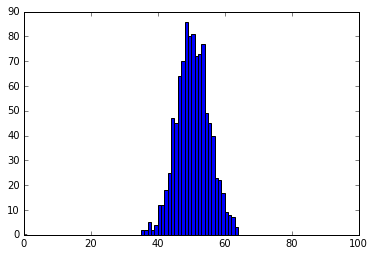
\includegraphics[height=7cm,keepaspectratio=true]{./pe/distBin01.png}
 % distBin01.png: 0x0 pixel, 300dpi, 0.00x0.00 cm, bb=
 \label{fig:2.10.1}
\end{figure}

\subsection{Normal Distribution}

One of the most important continuous probability distributions is the \emph{normal distribution}, also called the \emph{Gaussian distribution}, which is defined by the density function
\begin{align}
 \label{eq:2.10.4}
 f_{a,b}(x)=\dfrac{1}{\sqrt{2\pi}}e^{-\frac{1}{2}\frac{(x-a)^{2}}{b^{2}}}
\end{align}
where $a,b$ are specific parameters for each random variable $X.$

{Properties of the normal distribution}
If the r.v. $X$ has the density function given by \eqref{eq:2.10.4}, with parameters $a,b$, then
\begin{align}
 a = \mu_{X}\\
 b = \s_{X}
\end{align}

If a normal random variable $X$ has density function
\begin{align}
 \label{eq:2.10.4a}
 f(x)=\dfrac{1}{\sqrt{2\pi}}e^{-\frac{1}{2}\frac{(x-\mu)^{2}}{\s^{2}}},
\end{align}
we write $X\sim N(\mu, \s^{2}).$

{Standardized random variable}
\begin{align}
 \label{eq:2.10.5}
 Z = \dfrac{X-\mu}{\s}\\
 \mu_{Z}=0 \\
 \s_{Z}=1
\end{align}

{Standard Form}
\begin{align}
 \label{eq:2.10.6}
 f(z)=\dfrac{1}{\sqrt{2\pi}}e^{-\frac{1}{2}z^{2}}
\end{align}

In this case, we say that $Z$ is \emph{normally distributed.}

\lstinputlisting[language=Python]{../code/distribuciones-especiales/distribucionNormal.py}

\begin{figure}
 \centering
 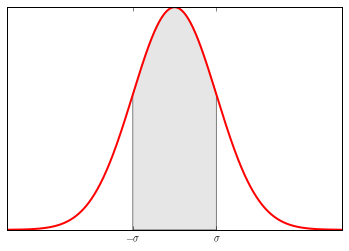
\includegraphics[height=5cm,keepaspectratio=true]{./pe/norm1.png}
 % norm1.png: 0x0 pixel, 300dpi, 0.00x0.00 cm, bb=
 \label{fig:2.10.2}
\end{figure}
\begin{verbatim}
 #(0.682689492137086, 7.579375928402476e-15)
\end{verbatim}

\begin{figure}
 \centering
 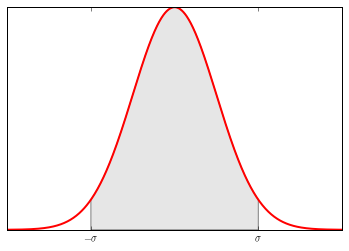
\includegraphics[height=5cm,keepaspectratio=true]{./pe/norm2.png}
 % norm1.png: 0x0 pixel, 300dpi, 0.00x0.00 cm, bb=
 \label{fig:2.10.3}
\end{figure}
\begin{verbatim}
 #(0.9544997361036417, 1.8403548653972355e-11)
\end{verbatim}

\begin{figure}
 \centering
 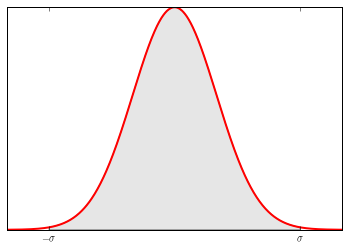
\includegraphics[height=5cm,keepaspectratio=true]{./pe/norm3.png}
 % norm1.png: 0x0 pixel, 300dpi, 0.00x0.00 cm, bb=
 \label{fig:2.10.4}
\end{figure}
\begin{verbatim}
 #(0.9973002039367399, 1.1072256503105314e-14)
\end{verbatim}

\begin{figure}
 \centering
 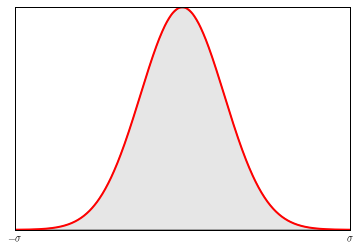
\includegraphics[height=5cm,keepaspectratio=true]{./pe/norm4.png}
 % norm1.png: 0x0 pixel, 300dpi, 0.00x0.00 cm, bb=
 \label{fig:2.10.5}
\end{figure}
\begin{verbatim}
 #(0.9999366575163339, 4.838904125482879e-12)
\end{verbatim}

\lstinputlisting[language=Python]{../code/distribuciones-especiales/normalCDF.py}
\begin{center}
 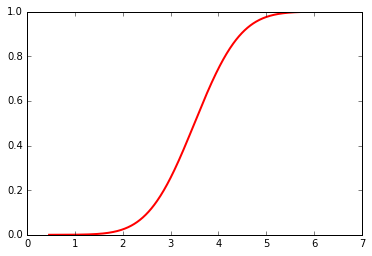
\includegraphics[height=5cm,keepaspectratio=true]{./pe/normCDF.png}
 % normCDF.png: 0x0 pixel, 300dpi, 0.00x0.00 cm, bb=
\end{center}

\subsection{Relationship Between the Binomial and Normal Distributions}

If $N\to \infty, p,q>>0,$ and $X$ has a binomial distribution with parameters $N,p$, then
\begin{align}
 \dfrac{X-Np}{\sqrt{Npq}} \sim N(0,1).
\end{align}

\begin{ejemplo}
  \label{exmp:2.10.4}
  Consider the experiment of tossing a coin 16 times. Repeat this experiment 1,000,000 times. Verify that this experiment can be modeled by a random variable with distribution $N(\mu=8,\sigma^{2}=4).$
\end{ejemplo}

\lstinputlisting[language=Python]{../code/distribuciones-especiales/relBinomNormal.py}
\begin{center}
 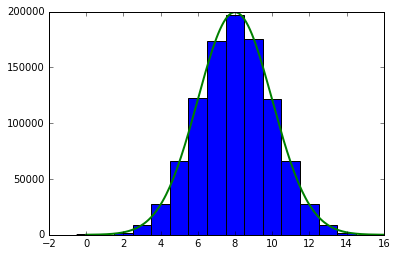
\includegraphics[height=5cm]{./pe/relBinNorm.png}
 % relBinNorm.png: 0x0 pixel, 300dpi, 0.00x0.00 cm, bb=
\end{center}

\subsection{The Poisson Distribution}
{Poisson Distribution} We say that a \emph{discrete} random variable $X$ has a Poisson distribution if its probability function is given by:
\begin{align}
 \label{eq:2.10.7}
 f(n)=\dfrac{\lam^{n}e^{-\lam}}{n!}, \; n=0,1,2,...
\end{align}

In this case, $\mu_{X}=\s^{2}=\lam.$

\begin{quote}
 In probability theory and statistics, the Poisson distribution is a discrete probability distribution that expresses, based on a mean frequency of occurrence, the probability of a given number of events occurring in a fixed interval of time or space. Specifically, it specializes in the probability of occurrence of rare events or events with very small probabilities.
\end{quote}

\href{https://en.wikipedia.org/wiki/Poisson_distribution}{Wikipedia: Poisson Distribution}

\begin{ejemplo}
  \label{exmp:2.10.5}
  The number of people arriving per day at an emergency room follows a Poisson distribution with mean 5. Find the probability that at most three arrive per day and the probability that at least 8 people arrive per day.
\end{ejemplo}

\begin{solucion}
	Using the Poisson distribution with $\lambda = 5$:
	
	\begin{enumerate}
		\item $P(X \leq 3) = \sum_{n=0}^{3} \frac{5^n e^{-5}}{n!}$
		\begin{align}
			&= \frac{5^0 e^{-5}}{0!} + \frac{5^1 e^{-5}}{1!} + \frac{5^2 e^{-5}}{2!} + \frac{5^3 e^{-5}}{3!} \\
			&= e^{-5}(1 + 5 + 12.5 + 20.833) \\
			&= e^{-5} \cdot 39.333 \approx 0.265
		\end{align}
		
		\item $P(X \geq 8) = 1 - P(X \leq 7)$
		\begin{align}
			&= 1 - \sum_{n=0}^{7} \frac{5^n e^{-5}}{n!} \\
			&\approx 1 - 0.867 = 0.133
		\end{align}
	\end{enumerate}
\end{solucion}

\lstinputlisting[language=Python]{../code/distribuciones-especiales/distPoisson.py}

\begin{figure}
 \centering
 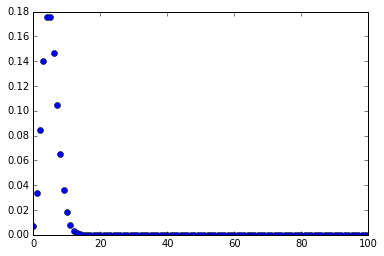
\includegraphics[height=7cm,keepaspectratio=true]{./pe/distPoisson0.png}
 % distPoisson0.png: 0x0 pixel, 300dpi, 0.00x0.00 cm, bb=
 \caption{Poisson Distribution}
\end{figure}

\begin{figure}
 \centering
 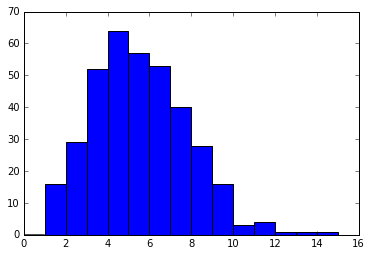
\includegraphics[height=7cm,keepaspectratio=true]{./pe/distPoisson1.png}
 % distPoisson1.png: 0x0 pixel, 300dpi, 0.00x0.00 cm, bb=
 \caption{Histogram of emergency room patients over a year with mean $\lam=5$}
 \label{fig:2.10.6}
\end{figure}

\subsection{Relationship Between the Binomial and Poisson Distributions}

If in the binomial probability function $N$ is very large while $p \approx 0,$ this models a \emph{rare event}. In practice, this means $N>>50, Np<<5.$

In this case, the binomial distribution with parameters $N,p$ approaches a Poisson distribution with parameter $\lam = Np.$

\lstinputlisting[language=Python]{../code/distribuciones-especiales/relBinomPoisson.py}

\begin{figure}
 \centering
 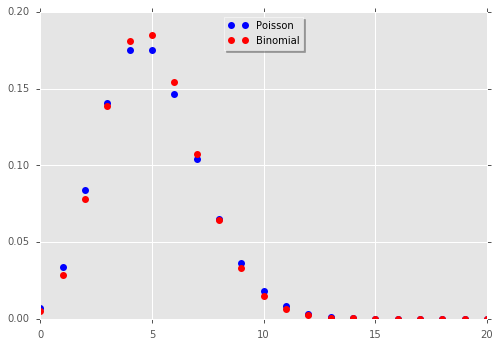
\includegraphics[height=7cm]{./pe/binVsPoi.png}
 % binVsPoi.png: 0x0 pixel, 300dpi, 0.00x0.00 cm, bb=
 \caption{Comparison between Binomial and Poisson distributions for rare events.}
\end{figure}

\subsection{Multinomial Distribution}

If events $E_{1},...,E_{k}$ can occur with probabilities $p_{1},...,p_{k}$ respectively, then the probability that they occur $X_{1},...,x_{k}$ times respectively is given by the \emph{multinomial distribution}
\begin{align}
 \label{eq:2.10.8}
 f\left( x_{1},...,x_{k} \right)=
 \dfrac{x_{1}+...+x_{k}}{x_{1}!...x_{k}!}p_{1}^{x_{1}}\cdots p_{k}^{x_{k}}.
\end{align}

\begin{ejemplo}
  \label{exmp:2.10.6}
  If a die is rolled 12 times, find the probability of obtaining each of the numbers $1,2,3,4,5,6$ exactly twice.
\end{ejemplo}

\begin{solucion}
	Using the multinomial distribution with $N=12$, $k=6$, $x_i = 2$ for all $i$, and $p_i = \frac{1}{6}$ for all $i$:
	
	\begin{align}
		P(X_1=2, X_2=2, ..., X_6=2) &= \frac{12!}{2! \cdot 2! \cdot 2! \cdot 2! \cdot 2! \cdot 2!} \left(\frac{1}{6}\right)^2 \cdots \left(\frac{1}{6}\right)^2 \\
		&= \frac{12!}{(2!)^6} \left(\frac{1}{6}\right)^{12} \\
		&= \frac{479001600}{64} \cdot \frac{1}{2176782336} \\
		&\approx 0.00344
	\end{align}
\end{solucion}

\subsection{Solved Problems}
{Percentile}
We say that $x=P_{q}$ is the $q$-th percentile ($0\leq q \leq 100$) of the distribution $F(x)$ if $F(P_{q})=q\%.$ If $q$ is an attainable value of $F(x),$ we can solve for
\begin{align}
 P_{q}=F^{-1}\left( \dfrac{q}{100} \right).
\end{align}
Such a function is called the \emph{inverse distribution function.}

{Quartiles}
Similar concepts are defined in the literature. For example, the first \emph{quartile} corresponds to the 25th percentile; the second quartile to the 50th percentile; and so on.

{Combinations}
\begin{ejemplo}
  \label{exmp:2.10.7}
  Find
  \begin{enumerate}
   \item $5!$
   \item $\comb{8}{3}$
  \end{enumerate}
  using \texttt{Python.}
\end{ejemplo}

\lstinputlisting[language=Python]{../code/distribuciones-especiales/combinaciones.py}

{Binomial Distribution}
\begin{ejemplo}
  \label{exmp:2.10.8}
  Suppose that $15\%$ of the population is left-handed. Find the probability that in a group of 50 individuals there are:
  \begin{enumerate}
   \item at most 10 left-handed individuals; 
   \item at least 5 left-handed individuals; 
   \item between 3 and 6 left-handed individuals; 
   \item exactly 5 left-handed individuals.
  \end{enumerate}
\end{ejemplo}

\lstinputlisting[language=Python]{../code/distribuciones-especiales/solvedBinom.py}

{Normal Distribution}
\begin{ejemplo}
  \label{exmp:2.10.9}
  On a final mathematics exam, the mean was 72 and the standard deviation was 15. Determine the standardized scores of students who obtained:
  \begin{enumerate}
   \item $60$;
   \item $93$;
   \item $72$.
  \end{enumerate}
\end{ejemplo}

\begin{ejemplo}
   \label{exmp:2.10.10}
   With the data from Problem \ref{exmp:2.10.9}, find the grades corresponding to the following standard scores:
  \begin{enumerate}
   \item $-1$;
   \item $1.6$.
  \end{enumerate}
\end{ejemplo}

\begin{ejemplo}
  \label{exmp:2.10.11}
  Suppose that the number of games played by major league baseball players during their career is normally distributed with a mean of $1500$ games and a standard deviation of $350$ games. Use \texttt{Python} to answer the following questions:
  \begin{enumerate}
   \item What percentage participate in fewer than 750 games?;
   \item what percentage participate in more than 2000 games?;
   \item find the $90$th \emph{percentile} of the number of games they play in their career.
  \end{enumerate}
\end{ejemplo}

\lstinputlisting[language=Python]{../code/distribuciones-especiales/solvedNorm.py}

{Rare Events}
\begin{ejemplo}
\label{exmp:2.10.12}
  If the probability that an individual suffers an adverse reaction from the injection of a certain serum is $0.001,$ determine the probability that among 2000 individuals:
 \begin{enumerate}
  \item exactly 3;
  \item more than 2
 \end{enumerate}
suffer an adverse reaction.
\end{ejemplo}

\lstinputlisting[language=Python]{../code/distribuciones-especiales/eventosRaros.py}

\subsection{The Geometric Distribution}

The geometric distribution models the number of independent Bernoulli trials needed to get the first success. If each trial has probability of success $p$ and probability of failure $q=1-p$, then the random variable $X$ that counts the number of trials up to and including the first success has probability function
\begin{align}
 \label{eq:2.10.9}
 f(k) = P(X=k) = (1-p)^{k-1}p, \quad k=1,2,3,\dots
\end{align}

A fundamental property of the geometric distribution is \emph{memorylessness}: the probability of obtaining a success in the next $k$ trials does not depend on the number of previous failures. That is, if $m,n\geq 1$,
\begin{align}
 P(X > m+n \mid X > m) = P(X > n).
\end{align}

{Properties of the geometric distribution} If $X$ has a geometric distribution with parameter $p$, then
\begin{align}
 \mu_{X} &= \dfrac{1}{p} \\
 \s_{X}^{2} &= \dfrac{1-p}{p^{2}}.
\end{align}

\begin{ejemplo}
 \label{exmp:2.10.13}
 A salesperson knows that the probability of closing a sale on any given telephone call is $p=0.2$. What is the probability that they need to make exactly $5$ calls to make the first sale? How many calls are expected on average?
\end{ejemplo}

\begin{solucion}
	Using the geometric distribution with $p=0.2$:
	\begin{align}
		P(X=5) &= (1-0.2)^{5-1}(0.2) = (0.8)^{4}(0.2) \\
		&= 0.4096 \times 0.2 = 0.08192
	\end{align}
	
	The expected number of calls is
	\begin{align}
		\mu = \dfrac{1}{p} = \dfrac{1}{0.2} = 5.
	\end{align}
\end{solucion}

\begin{ejemplo}
 \label{exmp:2.10.14}
 In a quality control process, the probability that a part is defective is $p=0.1$. What is the probability that the first defective part appears on the third inspection?
\end{ejemplo}

\lstinputlisting[language=Python]{../code/distribuciones-especiales/distGeom.py}

\begin{figure}
 \centering
 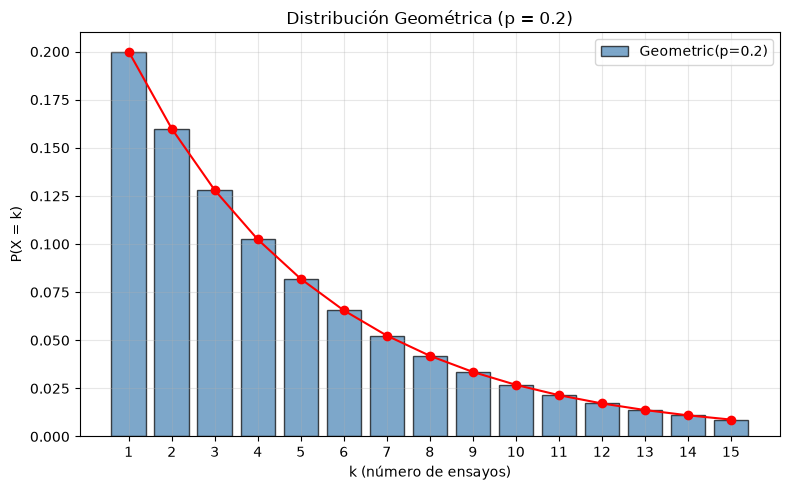
\includegraphics[height=7cm,keepaspectratio=true]{./pe/distGeom.png}
 % distGeom.png: 0x0 pixel, 300dpi, 0.00x0.00 cm, bb=
 \caption{Geometric distribution with $p=0.2$}
 \label{fig:2.10.7}
\end{figure}

\subsection{The Negative Binomial Distribution}

The negative binomial distribution generalizes the geometric distribution: it models the number of failures observed before obtaining a predetermined number $r$ of successes in a sequence of independent Bernoulli trials. Its probability function is given by
\begin{align}
 \label{eq:2.10.10}
 f(k) = P(X=k) = \binom{k+r-1}{r-1}p^{r}(1-p)^{k}, \quad k=0,1,2,\dots
\end{align}

Note that when $r=1$, the negative binomial reduces to the geometric distribution (counting failures before the first success).

{Properties of the negative binomial distribution} If $X$ has a negative binomial distribution with parameters $r$ and $p$, then
\begin{align}
 \mu_{X} &= \dfrac{r(1-p)}{p} \\
 \s_{X}^{2} &= \dfrac{r(1-p)}{p^{2}}.
\end{align}

\begin{ejemplo}
 \label{exmp:2.10.15}
 A certification exam has a pass rate of $30\%$. What is the probability that a student fails $4$ times before passing for the third time?
\end{ejemplo}

\begin{solucion}
	In this case, $r=3$ (number of successes) and $p=0.3$. The variable $X$ counts the number of failures before the third success.
	\begin{align}
		P(X=4) &= \binom{4+3-1}{3-1}(0.3)^{3}(0.7)^{4} \\
		&= \binom{6}{2}(0.027)(0.2401) \\
		&= 15 \times 0.027 \times 0.2401 \\
		&\approx 0.0972
	\end{align}
\end{solucion}

\lstinputlisting[language=Python]{../code/distribuciones-especiales/distNegBinom.py}

\begin{figure}
 \centering
 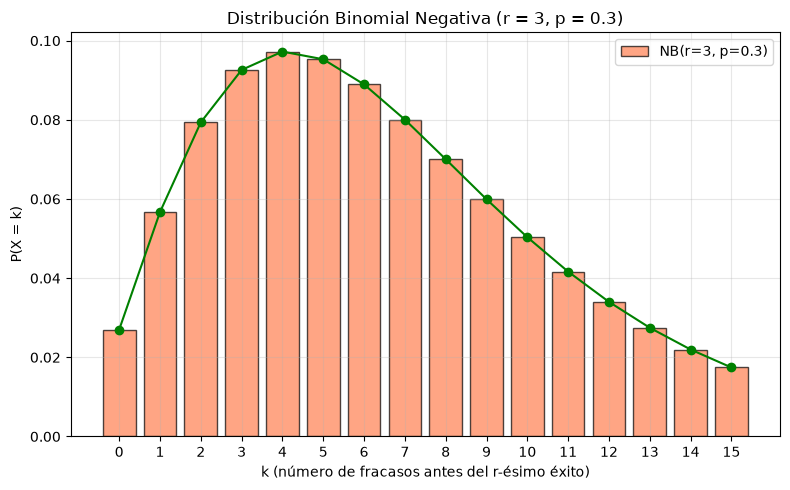
\includegraphics[height=7cm,keepaspectratio=true]{./pe/distNegBinom.png}
 % distNegBinom.png: 0x0 pixel, 300dpi, 0.00x0.00 cm, bb=
 \caption{Negative binomial distribution with $r=3$, $p=0.3$}
 \label{fig:2.10.8}
\end{figure}

\subsection{The Hypergeometric Distribution}

The hypergeometric distribution models the number of successes in $n$ draws \emph{without replacement} from a finite population of size $N$ that contains $K$ successes and $N-K$ failures. Its probability function is
\begin{align}
 \label{eq:2.10.11}
 f(k) = P(X=k) = \dfrac{\binom{K}{k}\binom{N-K}{n-k}}{\binom{N}{n}}, \quad \max(0, n-(N-K)) \leq k \leq \min(n, K).
\end{align}

Unlike the previous distributions, the trials here are \emph{not independent} because sampling without replacement changes the probabilities with each draw.

{Properties of the hypergeometric distribution} If $X$ has a hypergeometric distribution with parameters $N$, $K$, and $n$, then
\begin{align}
 \mu_{X} &= n\dfrac{K}{N} \\
 \s_{X}^{2} &= n\dfrac{K}{N}\dfrac{N-K}{N}\dfrac{N-n}{N-1}.
\end{align}

The factor $\dfrac{N-n}{N-1}$ is known as the \emph{finite population correction factor}. When $n \ll N$, this factor tends to $1$ and the hypergeometric distribution approaches the binomial with parameters $n$ and $p=K/N$.

\begin{ejemplo}
 \label{exmp:2.10.16}
 A batch contains $20$ items, of which $5$ are defective. If $4$ items are selected at random without replacement, what is the probability of finding exactly $2$ defective items?
\end{ejemplo}

\begin{solucion}
	Here $N=20$, $K=5$, $n=4$, $k=2$.
	\begin{align}
		P(X=2) &= \dfrac{\binom{5}{2}\binom{15}{2}}{\binom{20}{4}} \\
		&= \dfrac{10 \times 105}{4845} \\
		&= \dfrac{1050}{4845} \approx 0.2167
	\end{align}
\end{solucion}

\begin{ejemplo}
 \label{exmp:2.10.17}
 In a $5$-card poker hand dealt from a $52$-card deck, what is the probability of obtaining exactly $3$ kings?
\end{ejemplo}

\begin{solucion}
	Here $N=52$ (total cards), $K=4$ (kings), $n=5$ (cards in the hand), $k=3$.
	\begin{align}
		P(X=3) &= \dfrac{\binom{4}{3}\binom{48}{2}}{\binom{52}{5}} \\
		&= \dfrac{4 \times 1128}{2598960} \\
		&= \dfrac{4512}{2598960} \approx 0.00174
	\end{align}
\end{solucion}

\lstinputlisting[language=Python]{../code/distribuciones-especiales/distHyper.py}

\begin{figure}
 \centering
 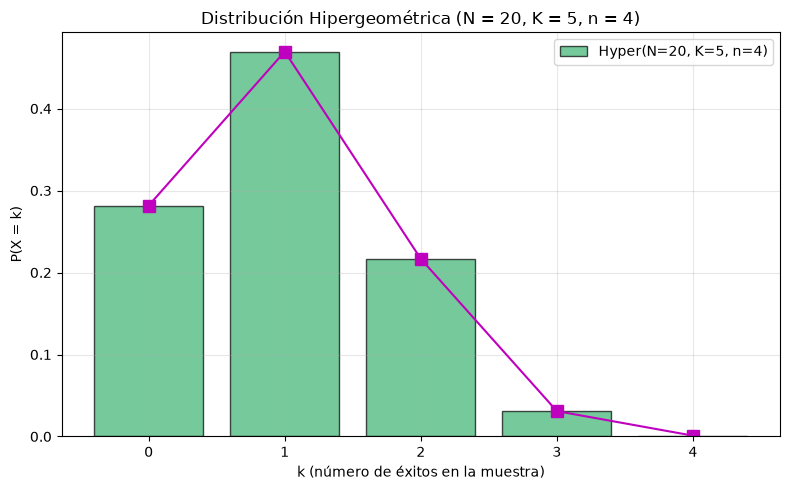
\includegraphics[height=7cm,keepaspectratio=true]{./pe/distHyper.png}
 % distHyper.png: 0x0 pixel, 300dpi, 0.00x0.00 cm, bb=
 \caption{Hypergeometric distribution with $N=20$, $K=5$, $n=4$}
 \label{fig:2.10.9}
\end{figure}

\begin{observacion}
	The hypergeometric distribution reduces to the binomial when sampling is done with replacement (or equivalently, as $N \to \infty$). In practice, if $\frac{n}{N} < 0.05$, the binomial approximation is reasonably accurate.
\end{observacion}

\subsection{Discrete Distributions and Their Relationship to Data Science}

The discrete distributions studied in this chapter are not merely theoretical objects: they are fundamental tools in data analysis and modeling. Below is a summary of their most common applications in data science.

\begin{itemize}
 \item \textbf{Binomial distribution:} Used in A/B testing to determine whether there is a statistically significant difference between two conversion rates. It is also the foundation of many binary classification models.
 
 \item \textbf{Poisson distribution:} Models the frequency of rare events in a fixed interval, such as the number of website visits per minute, customer service calls per hour, or manufacturing defects per unit. It is widely used in traffic analysis and anomaly detection.
 
 \item \textbf{Geometric distribution:} Models the number of trials up to the first success. In data science, it is applied in survival analysis (time until first conversion), churn modeling, and designing retention strategies.
 
 \item \textbf{Negative binomial distribution:} An extension of Poisson that allows modeling count data with \emph{overdispersion} (variance greater than the mean). It is common in real-world data where variability exceeds that predicted by Poisson, such as the number of transactions per customer or clicks per user.
 
 \item \textbf{Hypergeometric distribution:} Used when working with samples drawn without replacement from finite populations, such as quality audits, survey sampling, or exact statistical tests like Fisher's exact test.
\end{itemize}

\begin{ejemplo}
 \label{exmp:2.10.18}
 Suppose we want to analyze the number of clicks received by $100$ advertisements in one hour. The observed data have a mean $\bar{x}=4.2$ and variance $s^{2}=8.7$. Is it reasonable to model these data with a Poisson distribution?
\end{ejemplo}

\begin{solucion}
	In a Poisson distribution, the mean and the variance are equal: $\mu = \sigma^{2} = \lambda$. Since here $s^{2} = 8.7 \gg \bar{x} = 4.2$, the data exhibit \emph{overdispersion}. Therefore, a Poisson distribution is \emph{not} appropriate. Instead, using a negative binomial distribution is recommended, as it can model this additional variability.
\end{solucion}

\lstinputlisting[language=Python]{../code/distribuciones-especiales/distDataScience.py}

\begin{figure}
 \centering
 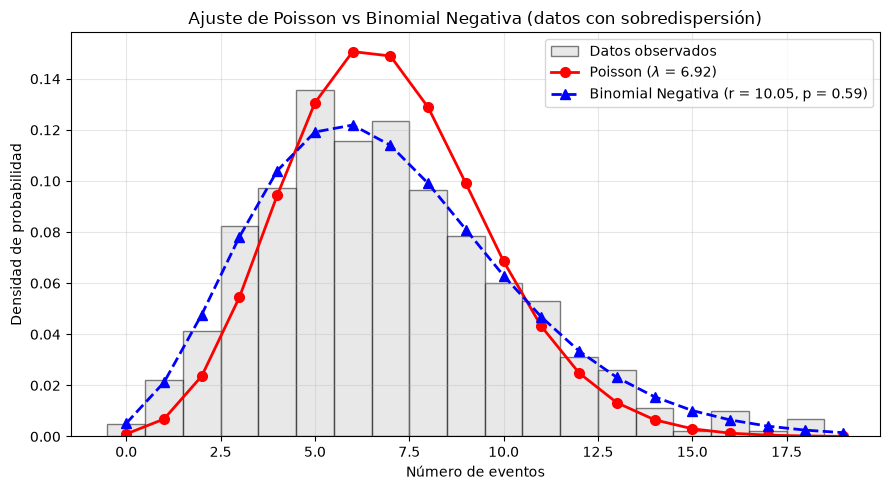
\includegraphics[height=7cm,keepaspectratio=true]{./pe/distDataScience.png}
 % distDataScience.png: 0x0 pixel, 300dpi, 0.00x0.00 cm, bb=
 \caption{Comparison of Poisson vs. Negative Binomial fit for overdispersed data}
 \label{fig:2.10.10}
\end{figure}

\begin{observacion}
	In practice, the choice of distribution depends on both the nature of the phenomenon being modeled and the statistical properties of the observed data. Tools such as the likelihood function, Akaike Information Criterion (AIC), and cross-validation allow us to compare different models and choose the most appropriate one.
\end{observacion}
